\chapter{System design and implementation}
\label{chapter:system-design}

This chapter presents the entire work of the author. The work is splitted in three parts for the attempt to combine deep neural networks with Q-Learning. The game chosen for experimenting was Tower of Hanoi due to its simplicity and also, the static environment. Then, the values obtained by Q-Learning were used to train a deep convolutional network in combination with the generated frames. Finally, we will try to combine Q-learning algorithm with convolutional networks.



\section{Q-Learning}

In this section we try to find the optimal policy for playing Tower of Hanoi game. The algorithm start with a pool of actions initialized with {UP, DOWN, LEFT, RIGHT} and a table Q which the values for all (state,action) pairs will be stored. 

The discount factor $\gamma$ is set to 0.95, this future rewards are taking into cosideration when updating the action-value function. The learning rate $\alpha$ is chosen to be 0.1, thus the algorithm can converge to an optimal policy. 

The exploration vs. exploitation problem is solved by using a variable $\epsilon$ which is initialized with 1 (1 is for choosing only random actions and 0 is for choosing the action that can maximize the score). For making the current policy to converge to the optimal policy there was also used a number of iterations setted to 11 and number of episodes per iteration setted to 1000. After each iteration is finished, $\epsilon$ is decreased with 0.1 until it will take the 0-value. This method was used to let the agent explore using random action in the first iteration and after exploit the values learned in the last iterations.

After all the iterations are finished, the algorithm generates a dataset. For each value stored in Q-table, it generates the frame from each coded state.

\begin{figure}[hp]
\centering
\minipage{0.32\textwidth}
  \frame{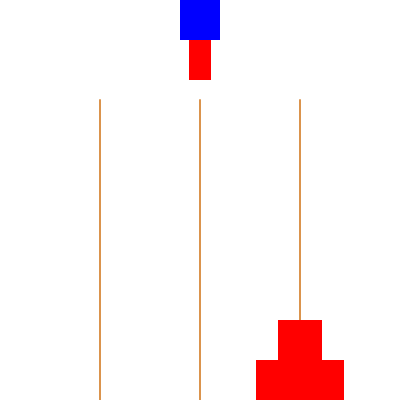
\includegraphics[width=\linewidth]{src/img/results/50}}
  \caption{\newline97,6530\newline100,0000\newline93,8538\newline92,5261}\label{fig:a}
\endminipage\hfill
\minipage{0.32\textwidth}
  \frame{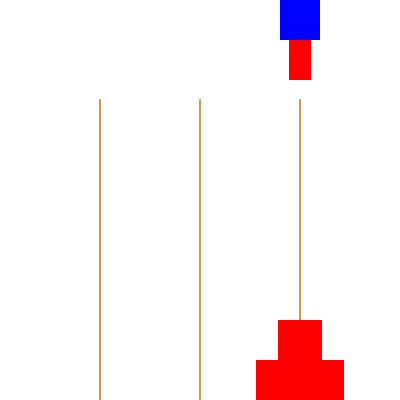
\includegraphics[width=\linewidth]{src/img/results/85}}
  \caption{\newline97,6530\newline100,0000\newline93,8538\newline92,5261}\label{fig:sc}
\endminipage\hfill
\minipage{0.32\textwidth}%
  \frame{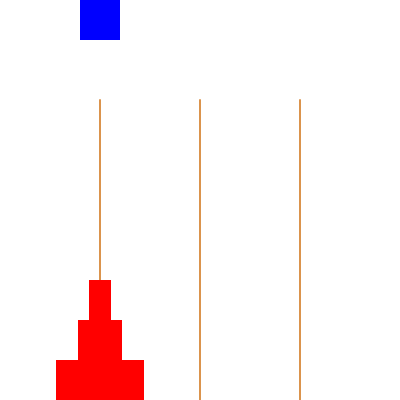
\includegraphics[width=\linewidth]{src/img/results/155}}
   \caption{\newline97,6530\newline100,0000\newline93,8538\newline92,5261}\label{fig:sc}
 
\endminipage
\end{figure}


\begin{algorithm}
	\floatname{algorithm}{Algorithm}
	\caption{Q-Network} \label{alg-code}
	\begin{algorithmic}[1]
		\State set size of Q to with no_states x no_action and initialize it
		\State choose $\epsilon$ between (0,1)
		\State let \textbf{s} be the current state of the game
		\State let \textbf{actions} be a pool with {$a_1$,$a_2$,...,$a_n$}
		\While{game not over}
			\State r = random number between (0,1)
			\If{r < $\epsilon$}
				\State $a_t$ = random action
			\Else
				\State $a_t$ = $argmax_a$ Q(s, a)
			\EndIf
			
			\State $s^\prime$, r = apply_action(a, s)
			\State Q(s,a) = Q(s,a) + $\alpha\cdot$(r + $\gamma\cdot \max_a Q(s^\prime,a^\prime)-Q(s,a)$)
		\EndWhile
	\end{algorithmic}
\end{algorithm}